\newpage
\section{Fast code}

As a \matlab{} beginner, it is quite easy to use code that just
works\texttrademark{} but comparing to compiled programs of higher programming
languages is very slow. The benefit of the relatively straightforward way of
programming in \matlab{} (where no such things as explicit memory allocation,
pointers, or data types ``come in your way'') needs to be paid with the
knowledge of how to avoid fundamental mistakes. Fortunately, there are only a
few \emph{big ones}, so when you browse through this section and stick to the
given hints, you can certainly be quite confident about your code.

\subsection{Using the profiler}

The first step in optimizing the speed of your program is finding out where it
is actually going slow. In traditional programming, bottlenecks are not quite
easily found, and the humble coder would maybe insert timer commands around
those chunks of code where he or she suspects the delay to actually measure
its performance. You can do the same thing in \matlab{} (using \lstinline!tic!
and \lstinline!toc! as timers) but there is a much more convenient way:
\emph{the profiler}.

The profiler is actually a wrapper around your whole program that measures the
execution time of each and every single line of code and depicts the result
graphically. This way, you can very quickly track down the lines that keep you
from going fast. See figure~\ref{figure:profiler} for an example output.

\begin{figure}
\centering
\begin{subfigure}[b]{0.45\textwidth}
  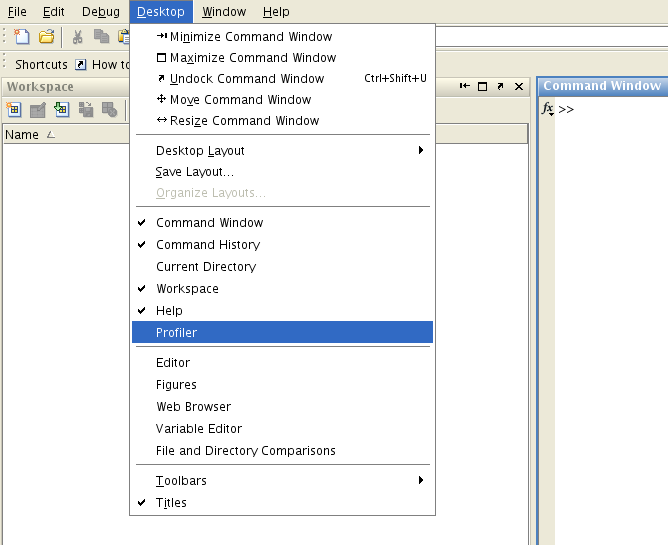
\includegraphics[height=5cm]{figures/matlab-open-profiler.png}
  \subcaption{Evoking the profiler through the graphical user interface.}
\end{subfigure}
\hfill
\begin{subfigure}[b]{0.45\textwidth}
  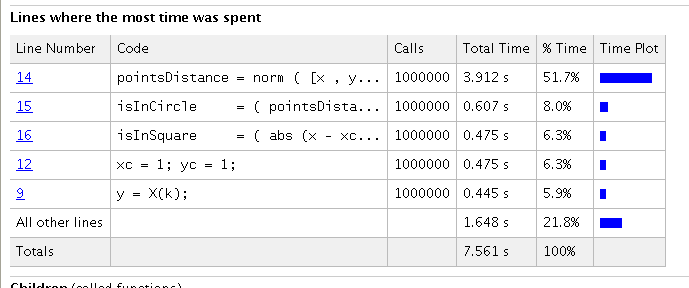
\includegraphics[width=6cm]{figures/matlab-profiler-circleBox-result.png}
  \subcaption{Part of the profiler output when running the routine of section
  on magic numbers (see page \pageref{example:magic-numbers}) one million
times. Clearly, the \lstinline!norm! command takes longest to execute, so when
trying to optimize one should start there.}
\end{subfigure}
\caption{Using the profiler.}
\label{figure:profiler}
\end{figure}

\begin{remark}
Besides the graphical interface, there is also a command line version of the
profiler that can be used to integrate it into your scripts. The commands to
invoke are \lstinline!profile on! for starting the profiler and
\lstinline!profile off! for stopping it, followed by various commands to
evaluate the gathers statistics. See the \matlab{} help page on
\lstinline!profile!.
\end{remark}


\subsection{The MATtrix LABoratory}

Contrary to common belief, the MAT in \matlab{} does not stand for mathematics,
but \emph{matrix}. The reason for that is that proper \matlab{} code uses
matrix and vector structures as often as possible, prominently at places where
higher programming languages such as C of Fortran would rather use loops.

The reason for that lies in \matlab{}'s being an interpreted language. That
means: There is no need for explicitly compiling the code, you just write it
and have in run. The \matlab{} interpreter then scans your code line by line
and executes the commands. As you might already suspect, this approach will
never be able to compete with compiled source code.

However, \matlab{}'s internals contain certain precompiled functions which
execute basic matrix-vector operations. Whenever the \matlab{} interpreter
bumps into a matrix-vector expression, the contents of the matrices are
forwarded to the underlying optimized and compiled code which, after
execution, returns the result. This approach makes sure that matrix operations
in \matlab{} are on par with matrix operations with compiled languages.

\begin{remark}
Not only for matrix-vector operations, precompiled binaries are provided. Most
standard tasks in numerical linear algebra are handled with a customized
version of the ATLAS (BLAS) library. This concerns for example commands such
as \lstinline!eig()! (for finding the eigenvalues of a matrix), \lstinline!\!
(for solving a linear equation system with Gau{\ss}ian\footnote{Johann Carl
Friedrich Gau{\ss} (1777--1855), German mathematician and deemed one of the
greatest mathematicians of all times. In the English-speaking world, the
spelling with `ss' instead of the original `\ss' has achieved wide acceptance
-- probably because the `\ss' is not included in the key set of any keyboard
layout except the German one.} elimination), and so on.
\end{remark}

\subsubsection{Matrix pre-allocation -- \fastsymbol\fastsymbol\fastsymbol\fastsymbol\fastsymbol}

When a matrix appears in \matlab{} code for the first time, its contents need to be
stored in system memory (RAM). To do this, \matlab{} needs to find a place in memory (a
range of \emph{addresses}) which is large enough to hold the matrix and assign this
place to the matrix. This process is called allocation. Note that, typically, matrices
are stored continuously in memory, and not split up to here and there. This way, the
processor can quickly access its entries without having to look around in the system
memory.

%  In some higher programming languages, the user needs to explicitly demand space allocation for an object, while in others do this automatically.

Now, what happens if the vector \lstinline!v! gets allocated with $55$
elements by, for example, \lstinline!v=rand(55,1)!, and the user decides later
in the code to make it a little bigger, say, \lstinline!v=rand(1100,1)!? Well,
obviously \matlab{} has to find a new slot in memory in case the old one is
not wide enough to old all the new entries. This is not so bad if it happens
once or twice, but can slow down your code dramatically when a matrix is
growing inside a loop, for example.


\hfill
\begin{minipage}[t]{.45\textwidth}
\begin{lstlisting}[framerule=2pt,rulecolor=\color{badred}]
n = 1e5;

for i = 1:n
    u(i) = sqrt(i);
end
\end{lstlisting}
The vector \lstinline!u! is growing \lstinline!n! times and it probably must be
re-allocated as often. The approximate execution time of this code snippet is
\extime{21.20}.
\end{minipage}
\hfill
\begin{minipage}[t]{.45\textwidth}
\begin{lstlisting}[framerule=2pt,rulecolor=\color{goodgreen}]
n = 1e5;
u = zeros(n,1);
for i = 1:n
    u(i) = sqrt(i);
end
\end{lstlisting}
As maximum size of the vector is known beforehand, one can easily tell
\matlab{} to place \lstinline!u! into memory with the appropriate size. The
code here merely takes \textbf{\SI{3.8}{\milli\second}} to execute!
\end{minipage}
\hfill

\begin{remark}
The previous code example is actually a little misleading as there is a much
quicker way to fill \lstinline!u! with the square roots of consecutive numbers.
Can you find the one-liner? A look into the next section could help\dots
\end{remark}


\subsubsection{Loop vectorization -- \fastsymbol\fastsymbol\fastsymbol\fastsymbol\fastsymbol}

Because of the reasons mentioned in the beginning of this section, you would
like to avoid loops wherever you can and try to replace it by a vectorized
operation.

When people commonly speak of `optimizing code for \matlab{}', it will most
often be this particular aspect. The topic is huge and this section can merely
give the idea of it. If you are stuck with slow loop operations and you have
no idea how to make it really quick, take a look at the excellent and
comprehensive guide at \cite{Mathworks:2009:CVG}. -- There is almost always a
way to vectorize.

Consider the following example a general scheme of how to remove loops from
vectorizable operations.

\hfill
\begin{minipage}[t]{.45\textwidth}
\begin{lstlisting}[framerule=2pt,rulecolor=\color{badred}]
n = 1e7;
a = 1;
b = 2;

x = zeros( n, 1 );
y = zeros( n, 1 );
for i=1:n
  x(i) = a + (b-a)/(n-1) ...
             * (i-1);
  y(i) = x(i) - sin(x(i))^2;
end
\end{lstlisting}
Computation of $f(x)=x-\sin^2(x)$ on \lstinline!n! points between \lstinline!a!
and \lstinline!b!. In this version, each and every single point is being
treated explicitly. Execution time: approx. \extime{0.91}.
\end{minipage}
\hfill
\begin{minipage}[t]{.45\textwidth}
\begin{lstlisting}[framerule=2pt,rulecolor=\color{goodgreen}]
n = 1e7;
a = 1;
b = 2;

h = 1/(n-1);


x = (a:h:b);

y = x - sin(x).^2;

\end{lstlisting}
Does the same thing using vector notation. Execution time: approx. \extime{0.12}.
\end{minipage}
\hfill

The \lstinline!sin()! function in \matlab{} hence takes a vector as argument
and acts as of it operated on each element of it. Almost all \matlab{}
functions have this capability, so make use of it if you can!


\paragraph{Vector indexing and boolean indexing.}\label{sec:logicalIndexing}
When dealing with vectors or matrices, it may sometimes happen that one has to
work only on certain entries of the object, e.g., those with odd index.

Consider the following three different possibilties of setting the \emph{odd}
entries of a vector \lstinline!v! to $0$.

\hfill
\begin{minipage}[t]{.29\textwidth}
\begin{lstlisting}[framerule=1pt,rulecolor=\color{goodgreen}]
% [...] create v

n = length(v);

for k = 1:2:n
  v(k) = 0;
end
\end{lstlisting}
Classical loop of the entries of interest (\extime{1.04}).
\end{minipage}
\hfill
\begin{minipage}[t]{.29\textwidth}
\begin{lstlisting}[framerule=1pt,rulecolor=\color{mediocre}]
% [...] create v

n = length(v);


v(1:2:n) = 0;

\end{lstlisting}
Vector indexing: Matrices take (positive) integer vectors as arguments
(\extime{1.14}).
\end{minipage}
\hfill
\begin{minipage}[t]{.29\textwidth}
\begin{lstlisting}[framerule=1pt,rulecolor=\color{badred}]
% [...] create v

n = length(v);
mask = false(n,1);
mask(1:2:n) =true;
v( mask ) = 0;

\end{lstlisting}
Boolean indexing: Matrices take \emph{boolean} arrays\footnotemark{} with the
same shape as \lstinline!v! as arguments (\extime{1.41}).
\end{minipage}
\hfill
\footnotetext{A mistake that beginners tend to make is to define
\lstinline!mask! as an array of integers, such as \lstinline!mask =
zeros(n,1);!.}

In this case, where the indices to be worked on are known beforehand, the
classical way of looping over the error is the fastest. Vector indexing makes
the code shorter, but creates a slight overhead; boolean indexing, by having to
create the boolean array \lstinline!mask!, is significantly slower.

However, should the criteria upon which action is taken dynamically depend on
the content of the vector itself, the situation is different.  Consider again
the three schemes, this time for setting the \lstinline!NaN! entries of a
vector \lstinline!v! to $0$.

\hfill
\begin{minipage}[t]{.29\textwidth}
\begin{lstlisting}[framerule=1pt,rulecolor=\color{badred}]
% [...] create v

for k = 1:n
  if isnan(v(k))
    v(k) = 0;
  end
end
\end{lstlisting}
Classical loop: \extime{1.19}.
\end{minipage}
\hfill
\begin{minipage}[t]{.29\textwidth}
\begin{lstlisting}[framerule=1pt,rulecolor=\color{mediocre}]
% [...] create v

ind = ...
  find(isnan(v));
v( ind ) = 0;


\end{lstlisting}
Vector indexing: \extime{0.44}.
\end{minipage}
\hfill
\begin{minipage}[t]{.29\textwidth}
\begin{lstlisting}[framerule=1pt,rulecolor=\color{goodgreen}]
% [...] create v

mask = isnan(v);

v( mask ) = 0;


\end{lstlisting}
Boolean indexing: \extime{0.33}.
\end{minipage}
\hfill

Iterating through the array \lstinline!v! and checking each element
individually means disregarding the ``MAT'' in \matlab{}. Making use of the
\lstinline!find()! function, it is possible to have \lstinline!isnan()! work on
the whole vector before setting the desired indices to 0 in one go. Even better
than that, doing away with the overhead that \lstinline!find()! creates, is to
use the boolean array that \lstinline!isnan()! returns to index \lstinline!v!
directly\footnote{Remember: You can combine several \lstinline!mask!s with the
logical operators \lstinline!&! (``and'') and \lstinline!|! (``or''). For
example, \lstinline!mask = isnan(v) | isinf(v);! is \lstinline!true! wherever
\lstinline!v! has a \lstinline!NaN! \emph{or} an \lstinline!Inf!.}.

See also \cite{Mathworks:2001:MIM}.

% \begin{remark}
% Of course, things can get somewhat more difficult to vectorize, for example when the commands within the loop make contain more than just `\lstinline!i!' or `\lstinline!i-1!' as index references like above. There is, however, almost always a way to vectorize. If you do not know further, see \cite{Mathworks:2009:CVG}.
% \end{remark}

% \begin{example}
% The task is to write a function that gets a vector \lstinline!u! as input which contains
% \end{example}

% \subsubsection{Referencing matrix elements}
% This hint is actually pretty similar to what is stated in the previous paragraph.
%
% One is sometimes confronted with the
%
% \Pointinghand\quad Useful functions: \lstinline!find!


\subsection{Solving a linear equation system -- \cleansymbol\cleansymbol\fastsymbol\fastsymbol\fastsymbol}
When being confronted with a standard linear equation system of the form
$Au=b$, the solution can be written down as $u = A^{-1}b$ if $A$ is regular. It
may now be quite seductive to translate this into \lstinline!u = inv(A)*b! in
\matlab{} notation. Though this step will certainly yield the correct solution
(neglecting round-off errors, which admittedly can be quite large in certain
cases), it would take quite a long time to execute. The reason for this is the
fact that the computer actually does more work then required. What you tell
\matlab{} to do here is to
\begin{enumerate}
\item explicitly calculate the inverse of \lstinline!A!, store it in a temporary matrix, and then
\item multiply the this matrix with \lstinline!u!.
\end{enumerate}
However, one is most often not interested in the explicit form of $A^{-1}$, but
only the final result $A^{-1}b$. The proper way out is \matlab{}'s
\lstinline!\! (backslash) operator (or equivalently \lstinline!mldivide()!)
which exactly serves the purpose of solving an equation system with Gau{\ss}ian
elimination.

% While computing a full inverse takes $O(n^4)$ operations (with $n$ being the
% dimension of the matrix), solving the equation system is as expensive as
% $O(n^3)$, so you definitely want to go with it.

\hfill
\begin{minipage}[t]{.45\textwidth}
\begin{lstlisting}[framerule=2pt,rulecolor=\color{badred}]
n = 2e3;
A = rand(n,n);
b = rand(n,1);

u = inv(A)*b;
\end{lstlisting}
Solving the equation system with an explicit inverse. Execution time: approx.
\extime{2.02}.
\end{minipage}
\hfill
\begin{minipage}[t]{.45\textwidth}
\begin{lstlisting}[framerule=2pt,rulecolor=\color{goodgreen}]
n = 2e3;
A = rand(n,n);
b = rand(n,1);

u = A\b;
\end{lstlisting}
Solving the equation system with the \lstinline!\! operator. Execution time: approx. \extime{0.80}.
\end{minipage}
\hfill

% The speed gain is actually not as ground-breaking as the order of magnitude
% points to; this suggests that \matlab{} actually has some build-in logic that
% works around this user's mistake. Still, using \lstinline!inv()! for solving
% an equation system in \matlab{} is considered a deadly sin in \matlab{} and
% should under all circumstances be avoided.


\subsection{Dense and sparse matrices -- \fastsymbol\fastsymbol\fastsymbol\fastsymbol\fastsymbol}

Most discretizations of particular problems yield $N\times N$-matrices which
only have a small number of non-zero elements (proportional to $N$). These are
called sparse matrices, and as they appear so very often, there is plenty of
literature describing how to make use of that structure.

In particular, one can
\begin{itemize}
\item cut down the amount of memory used to store the matrix. Of course,
  instead of storing all the $0$'s, one would rather store the value and
  indices of the non-zero elements in the matrix. There are different ways of
  doing so. \matlab{} internally uses the condensed-column format, and exposes
  the matrix to the user in indexed format.

\item optimize algorithms for the use with sparse matrices. As a matter of
  fact, most basic numerical operations (such as Gau{\ss}ian elimination,
  eigenvalue methods and so forth) can be reformulated for sparse matrices and
  save an enormous amount of computational time.
\end{itemize}

% For these reasons, it is highly recommended to allocate matrices as sparse
% when they really are. There are a couple of functions which assist building
% up a sparse matrix, most notably \lstinline!sparse!, \lstinline!spdiags!, and
% \lstinline!speye!.

Of course, operations which only involve sparse matrices will also return a
sparse matrix (such as matrix--matrix multiplication \lstinline!*!,
\lstinline!transpose!, \lstinline!kron!, and so forth).



\hfill
\begin{minipage}[t]{.45\textwidth}
\begin{lstlisting}[framerule=2pt,rulecolor=\color{badred}]
n = 1e4;
h = 1/(n+1);

A = zeros(n,n);
A(1,1) =  2;
A(1,2) = -1;
for i=2:n-1
    A(i,i-1) = -1;
    A(i,i  ) =  2;
    A(i,i+1) = -1;
end
A(n,n-1) = -1;
A(n,n)   =  2;

A = A / h^2;

% continued below
\end{lstlisting}
Creating the tridiagonal matrix $1/h^2\times\diag[-1, 2, -1]$ in dense format.
The code is bulky for what it does, and cannot use native matrix notation.
Execution time: \extime{0.67}.
\end{minipage}
\hfill
\begin{minipage}[t]{.45\textwidth}
\begin{lstlisting}[framerule=2pt,rulecolor=\color{goodgreen}]
n = 1e4;
h = 1/(n+1);

e = ones(n,1);
A = spdiags([-e 2*e -e],...
            [-1   0  1],...
             n, n );







A = A / h^2;

% continued below
\end{lstlisting}
The three-line equivalent using the sparse matrix format. The code is not only
shorter, easier to read, but also saves gigantic amounts of memory. Execution
time: \textbf{\SI{5.4}{\milli\second}}!
\end{minipage}
\hfill

\medskip

\hfill
\begin{minipage}[t]{.45\textwidth}
\begin{lstlisting}[framerule=2pt,rulecolor=\color{badred}]
% A in dense format
b = ones(n,1);
u = A\b;
\end{lstlisting}
Gau{\ss}ian elimination with a tridiagonal matrix in dense format. Execution
time: \extime{55.06}.
\end{minipage}
\hfill
\begin{minipage}[t]{.45\textwidth}
\begin{lstlisting}[framerule=2pt,rulecolor=\color{goodgreen}]
% A in sparse format
b = ones(n,1);
u = A\b;
\end{lstlisting}
The same syntax, with \lstinline!A! being sparse. Execution time: \textbf{\SI{0.36}{\milli\second}}!
\end{minipage}
\hfill

% \begin{remark}
% Of course, not all matrices are sparse.
% \end{remark}

\Pointinghand\hspace{1em} Useful functions: \lstinline!sparse()!, \lstinline!spdiags()!, \lstinline!speye()!, (\lstinline!kron()!),\dots



\subsection{Repeated solution of an equation system with the same matrix -- \fastsymbol\fastsymbol\fastsymbol\fastsymbol\fastsymbol}

It might happen sometimes that you need to solve an equation system a number of
times with the same matrix but different right-hand sides. When all the right
hand sides are immediately available, this can be achieved with with one
ordinary `\lstinline!\!' operation.

\hfill
\begin{minipage}[t]{.45\textwidth}
\begin{lstlisting}[framerule=2pt,rulecolor=\color{badred}]
n = 1e3;
k = 50;
A = rand(n,n);
B = rand(n,k);

u = zeros(n,k);

for i=1:k
    u(:,k) = A \ B(:,k);
end
\end{lstlisting}
Consecutively solving with a couple of right-hand sides. Execution time:
\extime{5.64}.
\end{minipage}
\hfill
\begin{minipage}[t]{.45\textwidth}
\begin{lstlisting}[framerule=2pt,rulecolor=\color{goodgreen}]
n = 1e3;
k = 50;
A = rand(n,n);
B = rand(n,k);




u = A \ B;

\end{lstlisting}
Solving with a number of right hand sides in one go. Execution time:
\extime{0.13}.
\end{minipage}
\hfill


If, on the other hand, you need to solve the system once to get the next
right-hand side (which is often the case with time-dependent differential
equations, for example), this approach will not work; you will indeed have to
solve the system in a loop. However, one would still want to use the
information from the previous steps; this can be done by first factoring $A$
into a product of a lower triangular matrix $L$ and an upper triangular matrix
$U$, and then instead of computing $A^{-1}u^{(k)}$ in each step, computing
$U^{-1}L^{-1}u^{(k)}$ (which is a lot cheaper.

\hfill
\begin{minipage}[t]{.45\textwidth}
\begin{lstlisting}[framerule=2pt,rulecolor=\color{badred}]
n = 2e3;
k = 50;
A = rand(n,n);

u = ones(n,1);


for i = 1:k
  u = A\u;
end
\end{lstlisting}
Computing $u = A^{-k}u_0$ by solving the equation systems in the ordinary way.
Execution time: \extime{38.94}.
\end{minipage}
\hfill
\begin{minipage}[t]{.45\textwidth}
\begin{lstlisting}[framerule=2pt,rulecolor=\color{goodgreen}]
n = 2e3;
k = 50;
A = rand(n,n);

u = ones(n,1);

[L,U] = lu( A );
for i = 1:k
  u = U\( L\u );
end
\end{lstlisting}
Computing $u = A^{-k}u_0$ by $LU$-factoring the matrix, then solving with the $LU$ factors. Execution time: \extime{5.35}. Of course, when increasing  the number $k$ of iterations, the speed gain compared to the `\lstinline!A\!' will  be more and more dramatic.
\end{minipage}
\hfill

\begin{remark}
For many matrices $A$ in the above example, the final result will be heavily corrupted with round-off errors such that after $k=50$ steps, the norm of the residual $\norm{u_0-A^ku}$, which ideally equals $0$, can be pretty large.
\end{remark}


\paragraph{Factorizing sparse matrices.}
When $LU$- or Cholesky-factorizing a \emph{sparse matrix}, the factor(s) are in
general not sparse anymore and can demand quite an amount of space in memory to
the point where no computer can cope with that anymore. The phenomenon of
having non-zero entries in the $LU$- or Cholesky-factors where the orginal
matrix had zeros is called \emph{fill-in} and has attracted a lot of attention
in the past 50 years. As a matter of fact, the success of iterative methods for
solving linear equation systems is largely thanks to this drawback.

Beyond using an iterative method to solve the system, the most popular way to
cope with fill-in is to try to re-order the matrix elements in such a way that
the new matrix induces less fill-in. Examples of re-ordering are \emph{Reverse
Cuthill-McKee} and \emph{Approximate Minimun Degree}. Both are implemented in
\matlab{} as \lstinline!colrcm()! and \lstinline!colamd()!, respectively (with
versions \lstinline!symrcm()! and \lstinline!symamd()! for symmetric matrices).

One can also leave all the fine-tuning to \matlab{} by executing
\lstinline!lu()! for sparse matrices with more output arguments; this will
return a factorization for the permuted and row-scaled  matrix $PR^{-1}AQ = LU$
(see \matlab{}'s help pages and example below) to reduce fill-in and increase
the stability of the algorithm.

\hfill
\begin{minipage}[t]{.45\textwidth}
\begin{lstlisting}[framerule=2pt,rulecolor=\color{badred}]
n = 2e3;
k = 50;

% get a non-singular nxn
% sparse matrix A:
% [...]

u = ones(n,1);

[L,U] = lu( A );
for i = 1:k
  u = U\( L\u );
end
\end{lstlisting}
Ordinary $LU$-factorization for a sparse matrix \lstinline!A!. The factors \lstinline!L! and \lstinline!U! are initialized as sparse matrices as well, but the fill-in phenomenon will undo this advantage. Execution time: \extime{4.31}.
\end{minipage}
\hfill
\begin{minipage}[t]{.45\textwidth}
\begin{lstlisting}[framerule=2pt,rulecolor=\color{goodgreen}]
n = 2e3;
k = 50;

% get a non-singular nxn
% sparse matrix A:
% [...]

u = ones(n,1);

[L,U,P,Q,R] = lu(A);
for i = 1:k
  u = Q*( U\(L\(P*(R\u))) );
end
\end{lstlisting}
$LU$-factoring with permutation and row-scaling. This version can use less
memory, execute faster, and provide more stability than the ordinary
$LU$-factorization. Execution time: \extime{0.07}.

This factorization is implicitly applied by \matlab{} when using the
`\lstinline!\!'-operator for solving a sparse system of equations \emph{once}.
\end{minipage}
\hfill
